\documentclass[tikz,border=3pt]{standalone}
\usepackage[utf8]{inputenc}
\usepackage[T1]{fontenc}
\usepackage{lmodern}
\renewcommand{\familydefault}{\sfdefault}
\usepackage{sansmath}\sansmath
\usepackage[american]{circuitikz}
\usepackage{pgfplots}\pgfplotsset{compat=1.18,/pgf/number format/use comma,/pgf/number format/1000 sep={.}}
\usetikzlibrary{arrows.meta,calc,positioning,decorations.pathmorphing,patterns}
% paleta del sitio
\definecolor{nar}{HTML}{E8680C}\definecolor{narc}{HTML}{FFB35C}\definecolor{hielo}{HTML}{FFF3E8}
\definecolor{tinta}{HTML}{1D1D1F}\definecolor{gris}{HTML}{6E6E73}\definecolor{lila}{HTML}{7C5CF0}
\definecolor{azul}{HTML}{2F6FD6}\definecolor{menta}{HTML}{17A673}\definecolor{coral}{HTML}{E8342A}
\ctikzset{bipoles/thickness=1.6}
\begin{document}
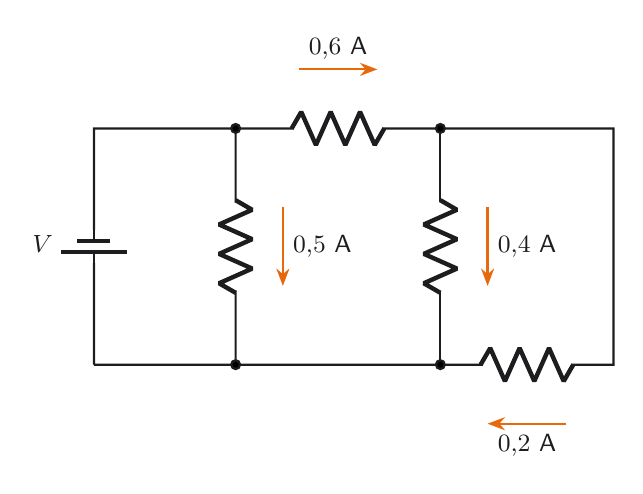
\begin{tikzpicture}[font=\small,>={Stealth[length=2.2mm]}]
\draw[tinta,thick] (0,0) to[battery1,l=$V$] (0,3) -- (1.8,3) to[R] (4.4,3) -- (6.6,3) -- (6.6,0) to[R] (4.4,0) -- (0,0);
\draw[tinta,thick] (1.8,3) to[R,*-*] (1.8,0);
\draw[tinta,thick] (4.4,3) to[R,*-*] (4.4,0);
\draw[->,nar,thick] (2.6,3.75) -- (3.6,3.75) node[midway,above,text=tinta] {$0{,}6$ A};
\draw[->,nar,thick] (2.4,2.0) -- (2.4,1.0) node[midway,right,text=tinta] {$0{,}5$ A};
\draw[->,nar,thick] (5.0,2.0) -- (5.0,1.0) node[midway,right,text=tinta] {$0{,}4$ A};
\draw[->,nar,thick] (6.0,-0.75) -- (5.0,-0.75) node[midway,below,text=tinta] {$0{,}2$ A};
\end{tikzpicture}
\end{document}
